\documentclass[tikz,border=5pt]{standalone}
\usepackage{pgfplots}
\pgfplotsset{compat=1.18}

\definecolor{corba}{HTML}{365FB3}
\definecolor{punt}{HTML}{B91C1C}
\definecolor{assimptota}{HTML}{6B7280}

\begin{document}
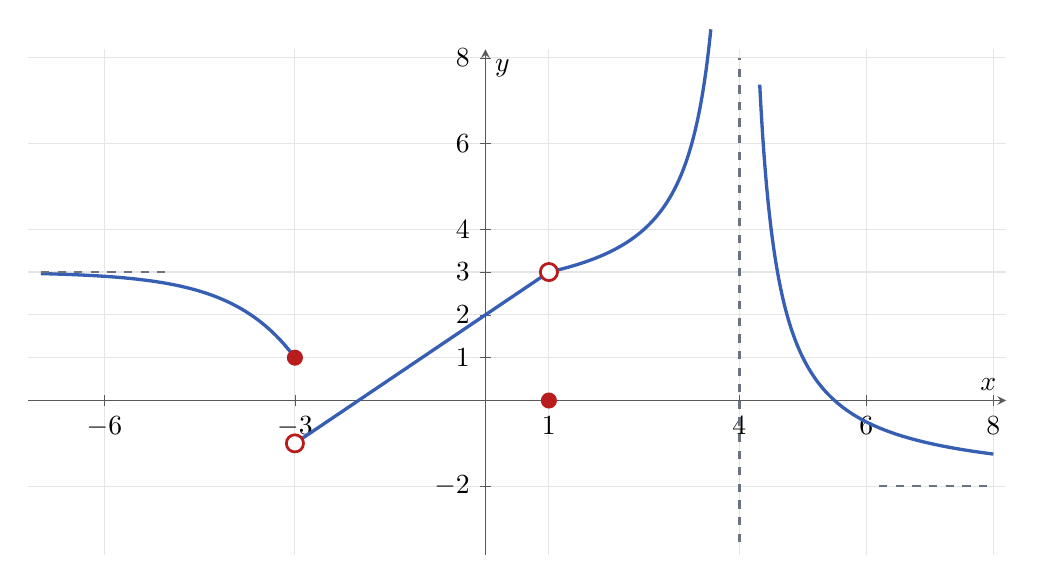
\begin{tikzpicture}
  \begin{axis}[
    width=14cm,
    height=8cm,
    axis lines=middle,
    xmin=-7.2,
    xmax=8.2,
    ymin=-3.6,
    ymax=8.2,
    xlabel={$x$},
    ylabel={$y$},
    xtick={-6,-3,0,1,4,6,8},
    ytick={-2,0,1,2,3,4,6,8},
    grid=major,
    grid style={black!10},
    axis line style={black!65},
    tick style={black!65},
    clip=false,
  ]
    % Branca esquerra: tendeix a y=3 i arriba a (-3,1).
    \addplot[corba, very thick, domain=-7:-3, samples=150]
      {3-2*exp(x+3)};

    % Tram lineal amb salt a x=-3 i forat a x=1.
    \addplot[corba, very thick, domain=-3:1, samples=2]
      {x+2};

    % Branca amb asímptota vertical a x=4.
    \addplot[corba, very thick, domain=1:3.55, samples=170]
      {2+3/(4-x)};
    \addplot[corba, very thick, domain=4.32:8, samples=170]
      {-2+3/(x-4)};

    % Asímptotes.
    \addplot[assimptota, dashed, thick, domain=-7:-5] {3};
    \draw[assimptota, dashed, thick]
      (axis cs:4,-3.3) -- (axis cs:4,8);
    \addplot[assimptota, dashed, thick, domain=6.2:8] {-2};

    % Punts oberts.
    \addplot[
      only marks,
      mark=*,
      mark size=3.1pt,
      mark options={draw=punt, fill=white, line width=1pt}
    ] coordinates {(-3,-1) (1,3)};

    % Punts definits.
    \addplot[
      only marks,
      mark=*,
      mark size=2.7pt,
      mark options={draw=punt, fill=punt}
    ] coordinates {(-3,1) (1,0)};
  \end{axis}
\end{tikzpicture}
\end{document}
